\documentclass[12pt]{article}
\usepackage[margin=1in]{geometry}                % See geometry.pdf to learn the layout options. There are lots.
\geometry{letterpaper}                   % ... or a4paper or a5paper or ... 
%\geometry{landscape}                % Activate for for rotated page geometry
\usepackage[parfill]{parskip}    % Activate to begin paragraphs with an empty line rather than an indent

%%%%%%%%%%%%%%%%%%%%
\newcommand{\hide}[1]{}



\usepackage{natbib}
\usepackage{xcolor}
\usepackage{url}
\usepackage{hyperref}
\usepackage{mathtools}
\usepackage[utf8]{inputenc}
\usepackage{float}
\usepackage{listings}
\usepackage{xcolor}
\usepackage{seqsplit}
\usepackage{verbatim}


\hide{
\usepackage{amscd}
\usepackage{amsfonts}
\usepackage{amsmath}
\usepackage{amssymb}
\usepackage{amsthm}
\usepackage{cases}		 
\usepackage{cutwin}
\usepackage{enumerate}
\usepackage{enumitem}
\usepackage{epstopdf}
\usepackage{graphicx}
\usepackage{ifthen}
\usepackage{lipsum}
\usepackage{mathrsfs}	
\usepackage{multimedia}
\usepackage{wrapfig}
}
\bibliographystyle{humanbio}


\usepackage[utf8]{inputenc}

\newcommand{\itemlist}[1]{\begin{itemize}#1\end{itemize}}
\newcommand{\enumlist}[1]{\begin{enumerate}#1\end{enumerate}}
\newcommand{\desclist}[1]{\begin{description}#1\end{description}}
\newcommand\tab[1][0.5cm]{\hspace*{#1}}

\newcommand{\Answer}[1]{\begin{quote}{\color{blue}#1}\end{quote}}
\newcommand{\AND}{\wedge}
\newcommand{\OR}{\vee}
\newcommand{\ra}{\rightarrow}
\newcommand{\lra}{\leftrightarrow}

\title {{\bf ECE 471 Lab 5} \\
\large{Packet Sniffing and Spoofing Lab / ARP Cache Poisoning Attack Lab
}}

\author{Mitchell Dzurick}
\date{4/15/2020}
\begin{document}

\maketitle
\textbf{Github with all documentation - \url{https://www.github.com/mitchdz/ECE471}}
\tableofcontents 
\clearpage



\section{Packet Sniffing and Spoofing Lab}

\subsection{Task 1.1: Sniffing Packets}
\subsubsection{Task 1.1A}
Wireshark is the most popular sniffing tool, and it is easy to use. We will use it throughout the entire lab.
However, it is difficult to use Wireshark as a building block to construct other tools. We will use Scapy
for that purpose. The objective of this task is to learn how to use Scapy to do packet sniffing in Python
programs. A sample code is provided in the following:
\begin{verbatim}
#!/usr/bin/python
from scapy.all import *

def print_pkt(pkt):
    pkt.show()

pkt = sniff(filter=’icmp’,prn=print_pkt)

\end{verbatim}

This code is placed into a file named sniffing.py and made executable with the following command

\begin{verbatim}
$ sudo chown +x sniffing.py
\end{verbatim}
The code can then be ran with the following command
\begin{verbatim}
$ ./sniffing.py
\end{verbatim}

The output after running as root is as follows:
\begin{figure}[H]
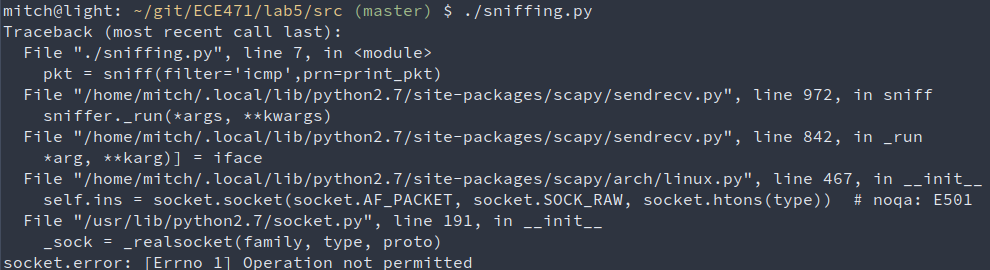
\includegraphics[scale=0.45]{images/p1t1_1.png}
\caption{Running the sniffing program without root}
\label{fig:p1t1_1}
\end{figure}

Looks like we need to utilize root to be able to run this script!

here's the output
\begin{verbatim}
<Sniffed: UDP:0 TCP:0 ICMP:2 Other:0>
\end{verbatim}

\subsubsection{Task 1.1b}
Task 1.1B. Usually, when we sniff packets, we are only interested certain types of packets. We can do
that by setting filters in sniffing. Scapy’s filter use the BPF (Berkeley Packet Filter) syntax; you can find the
BPF manual from the Internet. Please set the following filters and demonstrate your sniffer program again
(each filter should be set separately):
\begin{enumerate}
	\item Capture only the ICMP packet
	\item Capture any TCP packet that comes from a particular IP and with a destination port number 23.
	\item Capture packets comes from or to go to a particular subnet. You can pick any subnet, such as
	128.230.0.0/16; you should not pick the subnet that your VM is attached to.
\end{enumerate}



\subsection{Task 1.2: Spoofing ICMP Packets}
\subsection{Task 1.4: Sniffing and-then Spoofing (Extra Credit)}
In this task, you will combine the sniffing and spoofing techniques to implement the following sniff-and-
then-spoof program. You need two VMs on the same LAN. From VM A, you ping an IP X. This will
generate an ICMP echo request packet. If X is alive, the ping program will receive an echo reply, and
print out the response. Your sniff-and-then-spoof program runs on VM B, which monitors the LAN through
packet sniffing. Whenever it sees an ICMP echo request, regardless of what the target IP address is, your
program should immediately send out an echo reply using the packet spoofing technique. Therefore, regard-
less of whether machine X is alive or not, the ping program will always receive a reply, indicating that X
is alive. You need to use Scapy to do this task. In your report, you need to provide evidence to demonstrate
that your technique works.





\section{ARPCache Poisoning Attack Lab}
\subsection{Task 2.1: ARP Cache Poisoning}





\end{document}

